\documentclass{article}

\newif\iflotteryneurips
\ifdefined\LOTTERYNEURIPS
  \lotteryneuripstrue
\else
  \lotteryneuripsfalse
\fi

\iflotteryneurips
  \PassOptionsToPackage{numbers,compress}{natbib}
  \usepackage[main]{neurips_2026}
\else
  \usepackage[margin=1in]{geometry}
  \usepackage[numbers]{natbib}
\fi

\usepackage{booktabs}
\usepackage{graphicx}
\usepackage{amsmath}
\usepackage{amssymb}
\usepackage{xcolor}
\usepackage{hyperref}

\newif\iflotteryincludeappendix
\ifdefined\LOTTERYMAINONLY
  \lotteryincludeappendixfalse
\else
  \lotteryincludeappendixtrue
\fi

\iflotteryincludeappendix
  \newcommand{\cifarmovementappendixref}{Appendix Table~\ref{tab:cifar-movement-stats}}
\else
  \newcommand{\cifarmovementappendixref}{the supplemental generated movement table}
\fi

\title{Winning Tickets Are Not Posterior Modes:\\
Evidence from Posterior Support and Magnitude Controls}

\author{Anonymous}
\date{\today}

\begin{document}
\maketitle

\begin{abstract}
The lottery ticket hypothesis suggests that dense neural networks contain sparse
subnetworks that can be trained in isolation when rewound to their original
initialization. A tempting Bayesian interpretation is that these tickets
correspond to posterior modes, or to sparse supports induced by posterior
basins. We make this interpretation falsifiable: posterior-induced masks must
match IMP tickets better than local magnitude, dense-trajectory, and
pruning-process controls, not merely better than uniform random masks. Across
five-seed MNIST and Fashion-MNIST sparsity sweeps, and a CIFAR-10 ResNet-20
epoch-1 rewind setting where IMP exceeds dense accuracy, SGLD, SGHMC, cyclical
SGLD, SWAG, diagonal/KFAC Laplace, low-rank Hessian-plus-diagonal Laplace,
exact last-layer Laplace, selected/tensor-block full-covariance Laplace,
joint-group full-covariance Laplace, and subspace HMC all fail this stronger
criterion. Posterior supports often beat random masks, but they remain tied to
chain-start magnitude, dominated by dense magnitude, or closer to rewind
controls than to IMP. Direct mode/ticket audits agree: posterior samples can
match IMP tickets in logit or activation CKA while failing layer-sparsity and
Hamming-distribution thresholds, and their basin count does not match ticket
diversity. Mechanistic controls point instead to trajectory and pruning-process
structure: IMP-only residual support recovers much of the fixed-mask training
gap, while cross-seed transfer, posterior uncertainty, score-bin controls,
overlap-matched process controls, and tensor-matched round-exclusion
interventions do not rescue a posterior-mode account. In these settings,
winning tickets are trajectory and pruning-process objects, not Bayesian
posterior-mode supports. Exact dense full-network full-covariance CIFAR
posterior baselines remain an open limitation.
\end{abstract}

\section{Introduction}

The lottery ticket hypothesis (LTH) states that a dense randomly initialized
network contains sparse subnetworks that can be trained to match the dense
network when reset to their original initialization \citep{frankle2019lottery}.
This result raises a basic question about the object discovered by iterative
magnitude pruning (IMP): is a winning ticket a combinatorial artifact of the
optimization trajectory, or does it reflect a deeper probabilistic structure of
the posterior over weights?

A Bayesian reading is attractive. SGD and its noisy variants have long been
connected to approximate Bayesian inference \citep{welling2011sgld,
mandt2017sgd}. Bayesian deep learning further emphasizes that useful neural
network solutions are distributed across broad posterior regions rather than
isolated points \citep{wilson2020bayesian, izmailov2021posteriors}. If winning
tickets correspond to posterior modes or posterior-basin supports, LTH would be
evidence for a selection view of learning: pruning would reveal posterior
structure already present in the trained model.

This paper tests that interpretation directly. We ask:

\begin{quote}
Do posterior samples or posterior basins induce sparse supports that explain IMP
winning-ticket masks beyond dense magnitude, initialization magnitude, rewind
magnitude, chain-start magnitude, and pruning-process controls?
\end{quote}

The paper contributes three pieces of evidence. First, it states the
posterior-mode explanation as a support-equivalence claim with operational
gates: posterior-induced supports must beat local magnitude controls, not just
random masks, and mode/ticket distributions must match in both mask and
function space. Second, it evaluates these gates across repeated
MNIST/Fashion-MNIST sweeps and CIFAR-10 ResNet-20 posterior approximations,
including stochastic samplers, Laplace variants, SWAG, subspace HMC, and direct
mode/ticket distribution probes. Third, after the posterior account fails these
gates, it tests a mechanistic alternative: IMP tickets are better explained by
dense-trajectory and pruning-process structure, especially the IMP-only
residual support.

The conclusion is negative but scoped. Posterior masks beat random masks, but
they track the magnitude support of the dense checkpoint or the chain start.
When chains move, they move away from the chain start without moving toward the
IMP ticket. When function-space CKA is high, mask-distribution and basin-count
criteria still fail. When process controls are added, the strongest positive
signal is the IMP-selected residual, not a posterior-mode support.

\section{Related Work}

\paragraph{Lottery tickets and pruning.}
LTH was introduced by \citet{frankle2019lottery}. Follow-up work connected LTH
to rewinding and linear mode connectivity \citep{frankle2020linear}. Random
weighted networks with learned masks further emphasized the selection view of
learning \citep{ramanujan2020hidden}. Single-shot pruning methods such as SNIP
\citep{lee2019snip} and SynFlow \citep{tanaka2020synflow} provide important
non-Bayesian controls.

\paragraph{Mode connectivity and subspaces.}
Low-loss connectivity between neural network solutions challenges the view that
trained models are isolated modes \citep{garipov2018loss, draxler2018barriers}.
For lottery tickets specifically, \citet{paul2023unmasking} argue that IMP
masks encode axial subspaces that intersect matching linearly connected regions,
which is a direct non-Bayesian competitor to a posterior-mode explanation.
Permutation symmetries and re-basin methods further complicate parameter-space
mode counting \citep{entezari2022role, ainsworth2023git}. Our experiments
therefore include function-space clustering and linear barrier probes in
addition to mask overlap.

\paragraph{Bayesian neural networks.}
SGLD provides a simple route from SGD to approximate posterior sampling
\citep{welling2011sgld}. SGD itself can be interpreted as approximate Bayesian
inference in a stationary regime \citep{mandt2017sgd}. Practical posterior
approximations such as SWAG \citep{maddox2019swag} and exact small-model
sampling studies \citep{izmailov2021posteriors} show that posterior geometry is
structured and nontrivial. PAC-Bayesian and Bayesian LTH analyses
\citep{sakamoto2022pacbayes, kuhn2026bayesian} motivate the need for controls:
Bayesian language alone does not imply that IMP masks are posterior-mode
supports.

Our contribution is therefore not a new posterior approximation or a claim that
Bayesian inference is uninformative for pruning. It is a controlled
support-equivalence test: if posterior modes explain winning tickets, their
sparse supports should match IMP tickets after conditioning on dense magnitude,
rewind magnitude, trajectory magnitude, and pruning-process alternatives.

\section{Operational Test}

Let $m_{\mathrm{IMP}}$ denote the mask found by IMP at a fixed sparsity. For a
posterior sample $\theta^{(s)}$, the simplest posterior-induced mask is
\[
  m^{(s)} = \mathrm{TopK}(|\theta^{(s)}|),
\]
with the same number of kept weights as $m_{\mathrm{IMP}}$. We also construct
aggregate posterior masks from posterior mean, RMS, signal-to-noise ratio, high
variance, and low variance.

We compare all masks by support Jaccard similarity to $m_{\mathrm{IMP}}$:
\[
  J(m, m_{\mathrm{IMP}}) =
  \frac{|m \cap m_{\mathrm{IMP}}|}{|m \cup m_{\mathrm{IMP}}|}.
\]

The key controls are random same-sparsity masks, initialization magnitude
masks, dense trained magnitude masks, rewind magnitude masks, chain-start
magnitude masks for posterior chains, SNIP/SynFlow masks, fixed-mask retraining
controls, channel-aligned direct mode/ticket controls, and process-residual
interventions. The positive posterior-mode interpretation must satisfy a
stronger condition than beating random: posterior masks must explain IMP beyond
the chain-start, dense, rewind, trajectory, and process controls, and posterior
samples must move support in a way that increases IMP alignment.

\section{Current Results}

\subsection{Random Is Too Weak a Baseline}

Tables~\ref{tab:mnist-gate1} and~\ref{tab:fashion-gate1} show the current
Gate1 sparsity sweeps. Each row aggregates five seeds, three independent
dense-start SGLD chains per seed, and posterior masks at the matched IMP
sparsity.

\begin{table}[ht]
\centering
\caption{MNIST 5-seed Gate1 sparsity sweep. Posterior masks beat random but
fail against stronger controls at every sparsity. ``Post-Chain'' is the
Jaccard overlap between posterior masks and their chain-start magnitude masks.}
\label{tab:mnist-gate1}
\resizebox{\textwidth}{!}{%
\begin{tabular}{lrrrrrrrr}
\toprule
Config & Runs & Sparsity & Posterior & Random & Chain Start & Post-Chain & Dense Mag & Gate1 \\
\midrule
r2 p0.30 & 5 & 0.5100 & 0.3539 & 0.3246 & 0.3537 & 0.9303 & 0.8259 & Fail \\
r3 p0.30 & 5 & 0.6570 & 0.2669 & 0.2071 & 0.2670 & 0.9115 & 0.7258 & Fail \\
r5 p0.30 & 5 & 0.8319 & 0.2373 & 0.0918 & 0.2385 & 0.9298 & 0.5924 & Fail \\
r8 p0.30 & 5 & 0.9424 & 0.1275 & 0.0298 & 0.1275 & 0.9423 & 0.4028 & Fail \\
\bottomrule
\end{tabular}
}
\end{table}

\begin{table}[ht]
\centering
\caption{Fashion-MNIST 5-seed Gate1 sparsity sweep. The failure mode matches
MNIST. At the highest sparsity, IMP accuracy drops below the dense model, so
that row should be interpreted as a high-sparsity stress case.}
\label{tab:fashion-gate1}
\resizebox{\textwidth}{!}{%
\begin{tabular}{lrrrrrrrr}
\toprule
Config & Runs & Sparsity & Posterior & Random & Chain Start & Post-Chain & Dense Mag & Gate1 \\
\midrule
r2 p0.30 & 5 & 0.5100 & 0.3516 & 0.3246 & 0.3516 & 0.9314 & 0.7385 & Fail \\
r3 p0.30 & 5 & 0.6570 & 0.2595 & 0.2070 & 0.2594 & 0.9160 & 0.6378 & Fail \\
r5 p0.30 & 5 & 0.8319 & 0.2114 & 0.0917 & 0.2122 & 0.9212 & 0.5255 & Fail \\
r8 p0.30 & 5 & 0.9424 & 0.1300 & 0.0297 & 0.1300 & 0.9408 & 0.3813 & Fail \\
\bottomrule
\end{tabular}
}
\end{table}

\begin{figure}[t]
\centering
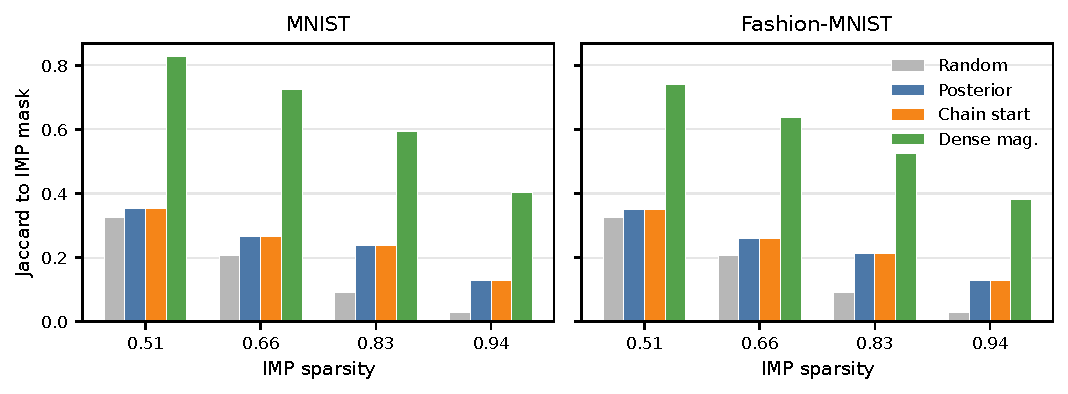
\includegraphics[width=\textwidth]{figures/gate1_controls.pdf}
\caption{Gate1 control comparison on MNIST and Fashion-MNIST. Posterior masks
beat random masks, but they track chain-start magnitude and remain far below
dense magnitude across sparsities.}
\label{fig:gate1-controls}
\end{figure}

Posterior masks beat random support at every tested MNIST/Fashion-MNIST
sparsity, but the random gap is explained by chain-start magnitude. On MNIST
and Fashion-MNIST, posterior-minus-chain-start gaps stay near zero while
posterior-to-chain-start overlap remains around 0.91--0.94. Dense magnitude is
much closer to IMP, with dense-minus-posterior gaps of 0.275--0.472 on MNIST
and 0.251--0.387 on Fashion-MNIST. The same pattern holds in the generated
mode-distribution audit: posterior supports beat uniform random masks in 58 of
59 grouped comparisons, but none of the 59 posterior-versus-chain-start
comparisons beats the matched chain-start support by more than 0.005 Jaccard:
43 are practically tied to the control, 15 favor chain-start magnitude, and one
is mixed. Rewind magnitude is closer to the IMP ticket than posterior support in
55 of 57 grouped comparisons.

\subsection{Sampler Movement Does Not Point Toward Tickets}

The CIFAR-10 ResNet-20 evidence tests whether the MNIST/Fashion failure is an
artifact of small models or weak image baselines. In the long-budget epoch-1
rewind row, dense accuracy is about 88.5\% and IMP reaches about 89.8\% at
83.2\% sparsity, yet SGLD, SGHMC, cyclical SGLD, SWAG, diagonal Laplace,
KFAC-style Laplace, low-rank Hessian-plus-diagonal Laplace, and subspace HMC
all fail the same control. Increasing sampler scale often lowers
posterior-to-chain-start overlap, but posterior-to-IMP overlap does not improve
and the epoch-1 rewind support remains closer to IMP.

\begin{figure}[t]
\centering
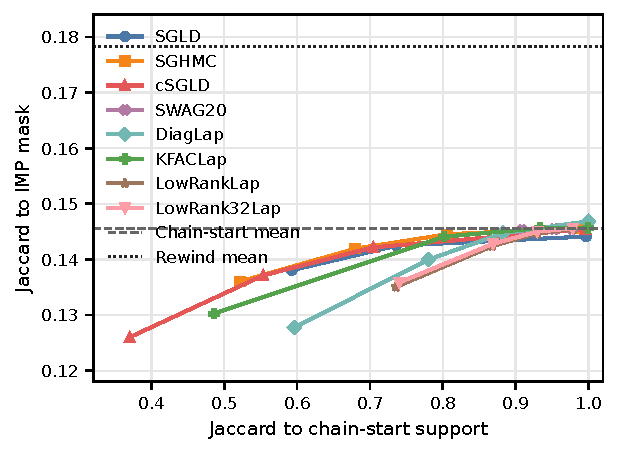
\includegraphics[width=0.72\textwidth]{figures/cifar_movement.pdf}
\caption{CIFAR-10 ResNet-20 epoch-1 rewind movement diagnostics. Across SGLD,
SGHMC, cyclical SGLD, full-network SWAG, diagonal Laplace, KFAC-style Laplace,
and low-rank Hessian-plus-diagonal Laplace, moving support away from the chain
start does not increase overlap with the IMP mask.}
\label{fig:cifar-movement}
\end{figure}

\begin{table}[t]
\centering
\small
\setlength{\tabcolsep}{3.5pt}
\begin{tabular}{llrrrrrr}
\toprule
Sampler & LR/Scale/Step & Dense & IMP & Post. & Chain & Post-chain & Rewind \\
\midrule
SGLD & $10^{-6}$ & 0.8845 & 0.8993 & 0.1425 & 0.1441 & 0.7362 & 0.1784 \\
SGLD & $3{\times}10^{-6}$ & 0.8845 & 0.8993 & 0.1381 & 0.1441 & 0.5928 & 0.1784 \\
cSGLD & $10^{-6}$ & 0.8852 & 0.8960 & 0.1422 & 0.1454 & 0.7046 & 0.1789 \\
DiagLap & $10^{-3}$ & 0.8849 & 0.8980 & 0.1447 & 0.1469 & 0.8826 & 0.1787 \\
DiagLap & $10^{-2}$ & 0.8849 & 0.8980 & 0.1278 & 0.1469 & 0.5961 & 0.1787 \\
KFACLap & $10^{-2}$ & 0.8860 & 0.8956 & 0.1303 & 0.1456 & 0.4859 & 0.1775 \\
LowRank32Lap & $10^{-2}$ & 0.8853 & 0.8964 & 0.1358 & 0.1457 & 0.7402 & 0.1795 \\
LowRank64Lap & $10^{-2}$ & 0.8874 & 0.8954 & 0.1339 & 0.1433 & 0.7397 & 0.1766 \\
LowRank128Lap & $10^{-2}$ & 0.8867 & 0.8967 & 0.1351 & 0.1453 & 0.7358 & 0.1780 \\
SWAG20 & $64$ & 0.8859 & 0.8973 & 0.1453 & 0.1455 & 0.9086 & 0.1782 \\
RandSubHMC & $3{\times}10^{-3}$ & 0.8866 & 0.8965 & 0.1440 & 0.1440 & 0.9766 & 0.1779 \\
TrajSubHMC & $10^{-3}$ & 0.8849 & 0.8961 & 0.2290 & 0.2292 & 0.9915 & 0.1792 \\
Hess16SubHMC & $3{\times}10^{-4}$ & 0.8873 & 0.8974 & 0.1468 & 0.1468 & 0.9994 & 0.1799 \\
Hess32SubHMC & $3{\times}10^{-4}$ & 0.8868 & 0.8973 & 0.1461 & 0.1461 & 0.9993 & 0.1788 \\
\bottomrule
\end{tabular}
\caption{Representative five-seed CIFAR-10 ResNet-20 epoch-1 rewind movement
diagnostics at r5 p0.30. Posterior support either remains near the chain-start
magnitude support or moves away from it, but posterior-to-IMP overlap (Post.)
does not exceed the matching chain-start control. TrajSubHMC is higher because
its chain-start control is the matched dense trajectory magnitude support; the
full generated movement summary is in \cifarmovementappendixref.}
\label{tab:cifar-long-movement}
\end{table}

The negative movement result is broad across posterior families. The sampler
grid includes dense-start and independent-start multi-chain SGLD, SGHMC,
cyclical SGLD, a 20-snapshot full-network SWAG movement row, diagonal and
KFAC-style Laplace, rank-16, rank-32, rank-64, and rank-128 top-Hessian
low-rank Laplace movement rows, exact final-head Laplace, selected and
tensor-block-diagonal full-covariance Laplace, joint-group Laplace, and
low-dimensional HMC in random, trajectory, and top-Hessian subspaces. Full-batch
HMC and an exact dense full-network Laplace sanity check on small digits MLPs
validate higher-fidelity small-model code paths while preserving the same
qualitative support failure.

\subsection{Richer Covariance Still Fails the Support Gate}

The covariance objection is the strongest bounded limitation. We therefore
push exact covariance as far as the workstation budget permits. We use a
22,064-parameter block-diagonal probe covering 22,064 trainable weights; at scale
$10^{-4}$ sample accuracy remains 88.1\%, global posterior-to-chain-start
support falls to 0.8287, the selected-block posterior-to-IMP support is below
the selected-block chain-start control by 0.0114 on average, the global
posterior-minus-chain gain is only 0.0036, and rewind remains closer by 0.0292.
Thus, this 22,064-parameter block-diagonal row moves support but not toward
tickets.

Wider exact covariance rows give the same answer, and this 68,144-parameter
block-diagonal row, covering 68,144 trainable weights, reports that sample accuracy remains
88.0\%, global support falls further to 0.7400, selected-block
posterior-minus-chain remains negative at -0.0050, global
posterior-minus-chain gain shrinks to 0.0010, and rewind remains closer by
0.0319, and this 68,144-parameter block-diagonal row remains negative. The
68,144-parameter joint-group row keeps the same 68,144 trainable
weights while including cross-tensor covariance inside groups; sample accuracy
remains 88.1\%, global posterior-to-chain-start support falls to 0.7148, block
posterior-minus-chain remains -0.0050, global posterior-minus-chain is 0.0015,
and rewind remains closer by 0.0311, so this 68,144-parameter joint-group row
also fails. The next row is this 86,576-parameter joint-group row,
covering 86,576 trainable weights, and it preserves sample accuracy at 88.3\%; global
posterior-to-chain-start support is 0.7863, block posterior-minus-chain stays
negative at -0.0023, global posterior-minus-chain stays 0.0006, and rewind
remains closer by 0.0317. The largest row is this 270,896-parameter joint-group row and covers
all 270,896 weight parameters; sample accuracy remains 88.2\%, global
posterior-to-chain-start support is 0.7389, block posterior-minus-chain remains
negative at -0.0019, global posterior-minus-chain is -0.0019, and rewind
remains closer by 0.0362. These rows remove the practical weight-tensor coverage
objection, while literal dense CIFAR full-network covariance remains outside
budget: a single float64 dense matrix would require 553.1 GiB, and matrix plus
Cholesky would require 1,106.3 GiB.

\subsection{Function Space Agreement Is Not Mask Equivalence}

We also make the original proposal's distributional criterion explicit. On
digits, posterior sample masks fail two of the four stated thresholds:
layer-sparsity KS has $p=0.0788$ and pairwise mask-Hamming overlap is 0.631,
while logit CKA passes. Mean-shift clustering in raw parameter PCA collapses
posterior samples to one representative mode; the raw-parameter basin entropy is
0.0 nats with effective cluster count 1.0. The full-data CIFAR-10 ResNet-20
strengthens this separation: posterior samples can keep logit/final-hidden
activation CKA above 0.93/0.91 while failing layer-sparsity, Hamming, or
posterior-basin-count criteria.

Alignment and stronger direct posterior probes do not change this conclusion:
activation-channel alignment are insufficient. The activation-aligned CIFAR row
still fails layer KS and Hamming while retaining high activation CKA.
Weight-correlation channel alignment reaches the same conclusion. The saved
artifact rerun supports record-level post-hoc matching, and a block-coordinate
ResNet channel audit still leaves global-channel posterior/ticket Hamming near
0.21 rather than ticket-like agreement. An exact stage-1 enumeration validates
the local solver on a small ResNet subgraph, while exhaustive full-data graph
isomorphism remains infeasible.

The multi-chain and high-fidelity direct rows address the concern that a single
local chain was too weak. A dense-start direct probe with 75 cyclical-SGLD
posterior samples fails layer KS and Hamming while maintaining high CKA; an
independent-start version with 15 dense chain starts and 75 samples does the
same. The rank-128 Hessian-plus-diagonal direct probe is the partial exception:
50 posterior samples now pass the Hamming-overlap threshold (0.816) and retain
high logit/final-hidden activation CKA (0.932/0.910), but still fail the
layer-sparsity KS threshold ($p=2.0{\times}10^{-6}$), and all 50 samples still
collapse to one parameter-PCA basin. A streamed exact joint-group direct probe
over the same all 270,896 weight parameters closes the full-weight Gaussian
gap: 25 joint-group posterior samples keep sample accuracy remains 88.3\%,
posterior-to-chain-start Hamming is 0.0503, layer-sparsity KS is
$p=1.1{\times}10^{-8}$, Hamming overlap is 0.000, logit/final-hidden activation
CKA remains 0.937/0.920, and All 25 joint-group samples still collapse to one
parameter-PCA basin.

\subsection{IMP Residuals Are Process Objects}

Posterior failure leaves a positive mechanism to explain. Dense trajectory
magnitude is useful: in the matched CIFAR dense-trajectory probe, trajectory
magnitude supports are closer to IMP than posterior supports, and fixed-mask
training shows that final dense, epoch-10, and RMS trajectory masks are much
better than random. They are still below IMP, so the remaining question is what
IMP adds.

\begin{figure}[t]
\centering
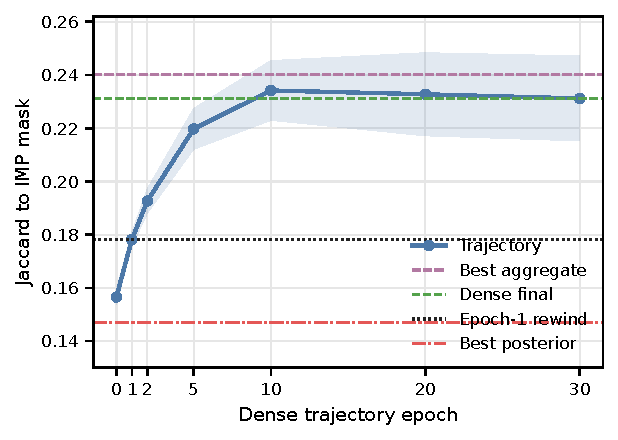
\includegraphics[width=0.70\textwidth]{figures/cifar_trajectory.pdf}
\caption{CIFAR-10 ResNet-20 dense-trajectory controls. Magnitude supports along
the matched dense trajectory, especially around epochs 10--30, and the best
aggregate trajectory magnitude score are closer to the IMP mask than any global
posterior support in the movement diagnostics.}
\label{fig:cifar-trajectory}
\end{figure}

Residual swap and removal-order controls localize the gap to a
process-selected IMP-only residual. Anatomy, predictor-mask, cross-seed,
direct-transfer, base-compatibility, posterior-ordering, and stratified
controls give the same localization. Learned mask baselines do not replace that
residual: Gem-Miner-style, Bernoulli/Concrete variational pruning, and the
hard-concrete L0 gate baseline are below IMP in the current CIFAR
support/accuracy rows and do not rescue the calibration/OOD tradeoff. Their
learned objective can change uncertainty behavior, but not into a
ticket-support explanation.

The strongest process controls test whether simpler score composition explains
the residual. A tensor matched excluded oracle is still below the round-selected
IMP residual, and a tensor+score matched excluded oracle remains below it even
after matching parameter tensor and within-tensor round-score deciles. A
residualized round-score projection shows that removing base, dense-final, and
final-IMP magnitude subspaces reduces both accuracy and oracle overlap. The
original posterior-projection round-selected row reaches 88.47\% accuracy. A
posterior-residualized row reaches 88.25\% after additionally residualizing
against diagonal-Laplace posterior RMS, posterior standard deviation, and
posterior RMS-minus-dense features; the gap is 0.23 percentage points, 5/5
positive seeds with 95\% CI $[-0.03,0.48]$, and overlap drops from 0.6773 to
0.4850, a 0.1923 paired drop with 5/5 positive seeds. The diagonal-Laplace
posterior score subspace does not explain away the process signal. Finally, the learned
trajectory/process subspace check gives the cleanest compact result: the
round-selected row reaches 88.69\% accuracy, the learned-subspace residualized
row reaches 88.21\%, the gap is 0.48 percentage points, 5/5 positive seeds with
95\% CI $[0.29,0.67]$, and oracle overlap falls from 0.6807 to 0.4917, a
0.1890 learned-subspace paired drop. Thus the current learned process subspace
captures broad directions but does not substitute for the particular residual
coordinates selected by IMP.

\section{Discussion}

These results constrain a simple Bayesian interpretation of lottery tickets.
The posterior signal exists in a weak sense: posterior-induced masks are not
random. But this is not enough. The same signal is already present in the dense,
rewind, trajectory, or chain-start magnitude support. The explicit
distribution-equivalence audit turns this into a negative result rather than a
visual or single-metric impression: posterior support distributions separate
from random masks, yet they are tied to or worse than local magnitude controls
across the posterior families tested here. The evidence therefore favors a
trajectory/magnitude subspace account plus a process-selected residual over a
posterior-mode account.

This conclusion is compatible with mode-connectivity results. Independent
solutions can occupy separated regions in parameter or function space, and yet
the sparse supports induced by local posterior samples need not explain the IMP
ticket. A generated linear connectivity audit makes this point concrete. On
MNIST and Fashion-MNIST, dense-to-IMP linear barriers are nearly zero (0.0026
and 0.0395), but posterior support remains slightly below the chain-start
magnitude control. On CIFAR-10 ResNet-20, the long SGLD and SWAG dense-to-IMP
barriers are large (3.0827 and 3.7402), but posterior support is still tied to
chain-start support. Thus linear barriers are orthogonal landscape diagnostics,
not evidence of posterior-ticket equivalence.

\paragraph{Scope of the claim.}
The claim is not that Bayesian neural-network posteriors are useless, nor that
no posterior approximation could ever correlate with IMP coordinates. The claim
is narrower: under the posterior families and CIFAR-10/MNIST/Fashion-MNIST
settings tested here, posterior-induced sparse supports do not satisfy the
support-equivalence claim once dense, rewind, trajectory, and pruning-process
controls are included. The positive evidence in the paper is the alternative
localization: useful ticket structure is better explained by trajectory
magnitude plus a process-selected IMP residual.

\section{Limitations and Next Experiments}

The evidence is broad, but the paper should still be read as a controlled
negative result under the posterior approximations we can currently test, not
as a theorem about all Bayesian neural-network posteriors. The main limitations
are:

\begin{itemize}
  \item alignment robustness. Activation-channel alignment, weight-correlation
  channel alignment, record-level post-hoc matching, a block-coordinate global
  channel audit, and exact stage-1 enumeration are negative or bounded, but
  exhaustive full-data graph isomorphism remains infeasible and unimplemented;
  \item full-network exact/full-covariance Laplace or another still broader
  high-fidelity posterior baseline. Current evidence includes multi-chain
  cyclical SGLD, rank-128 low-rank Laplace, all-weight joint-group Laplace,
  20-snapshot SWAG, low-rank Hessian-plus-diagonal Laplace, tensor-block and
  joint-group full-covariance probes, and subspace HMC, but the exact dense
  full-network CIFAR posterior remains absent;
  \item broader learned-mask distribution variants. Gem-Miner-style score
  training, Bernoulli/Concrete variational pruning, and hard-concrete L0 gates
  do not rescue support, accuracy, calibration, or CIFAR-100 OOD behavior in
  the current five-seed rows, but additional permutation-aware learned-mask
  distributions would make this negative claim cleaner;
  \item additional process-causality controls. The current residual-swap,
  anatomy, predictor-mask, transfer, base compatibility, ordering,
  stratification, IMP-process, tensor+score-matched round-exclusion,
  residualized-score projection, posterior-residualized, and learned-subspace
  residualized controls do not exhaust the possible causal interventions on the
  pruning process;
  \item reproducibility hardening. The repository has a dependency list,
  checked environment lock, Makefile targets, artifact verifier, CI workflow,
  public release manifest, local release archive, source-only repository
  snapshot, CPU artifact-verification container, GPU training-container
  definition, external-validation runbook, and submission handoff. It still
  lacks public archive, public repository, external CI, and external GPU-run
  receipts.
\end{itemize}

Since the aligned, multi-chain, low-rank Laplace, and block or joint-group
Laplace CIFAR runs preserve the current pattern, the next decisive empirical
gap is an even stronger high-fidelity posterior baseline. If that baseline also
stays near the chain-start/rewind controls, the negative result is the right
paper: posterior samples reveal local magnitude structure, not IMP ticket
structure. If it contradicts the current pattern, the claim should be weakened
to a partial-equivalence statement that isolates the architectures, sparsities,
and posterior approximations where the Bayesian account survives.

\clearpage
\bibliographystyle{plainnat}
\bibliography{refs}

\iflotteryincludeappendix
  \clearpage
  \appendix
  \section{Generated Evidence Tables}

  \input{tables/statistical_summary.tex}
\fi

\iflotteryneurips
  \clearpage
  \input{neurips_checklist.tex}
\fi

\end{document}
